\chapter{Multicopter control realization}\label{sec:MulticopterRealization}

\begin{figure}
 \centering
 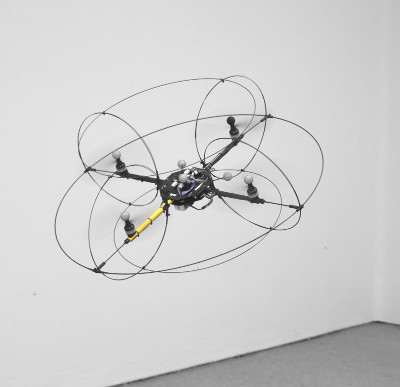
\includegraphics[height=5.5cm]{QuadV4.jpg}
 \hspace{.05\linewidth}
 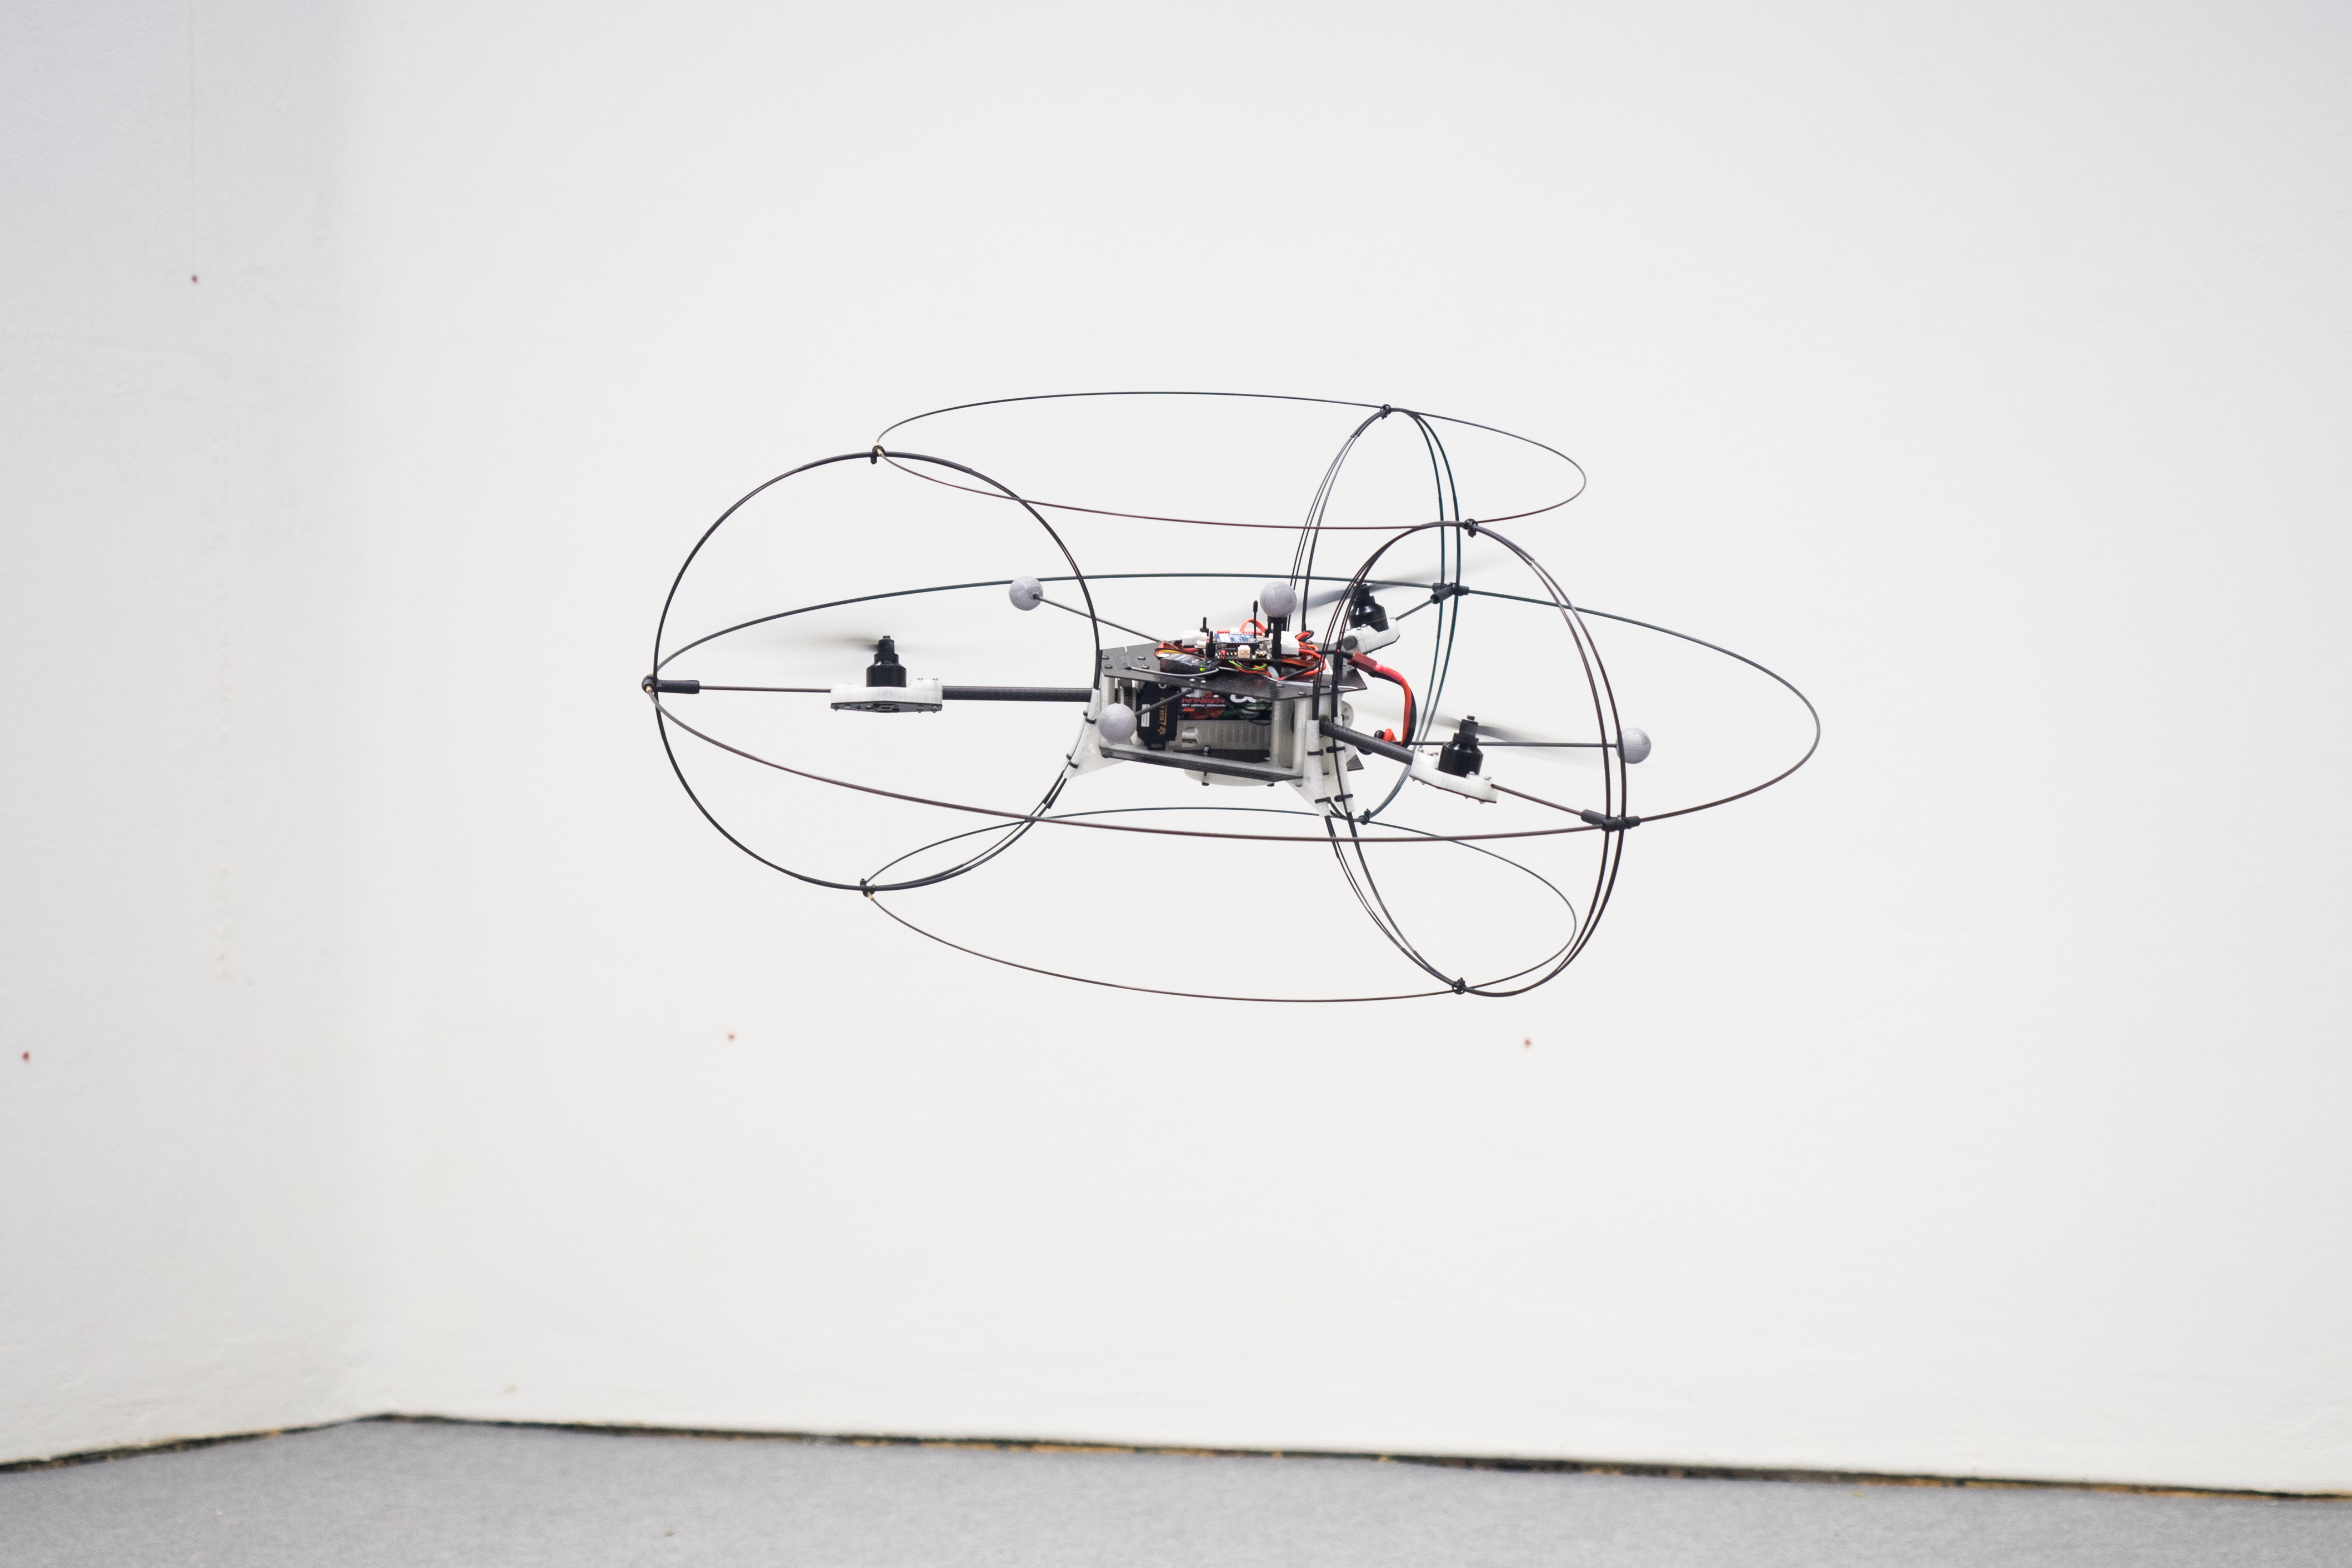
\includegraphics[height=5.5cm]{TriV4.jpg}
 \caption{LSR-Quad- and Tricopter}
 \label{fig:LSRQuadAndTri}
\end{figure}

This chapter describes the realization and discusses the experimental results with the LSR-Multicopters, \autoref{fig:LSRQuadAndTri}.
On the highest abstraction layer they can be regarded as a single rigid body with body fixed forces (the propeller forces and torques).
As such they are used for practical validation of the modeling and control approaches of the previous chapters.

The LSR-quadcopter started as a student project in 2009, a time in which they were not as ubiquitous as these drones are nowadays, 15 years later.
The original hardware, a kit from the online shop \url{www.mikrokopter.de}, was continuously improved and adapted for specific experiments until the only remaining original parts in 2018 were the motors and propellers.
The final version has an outer diameter of $0.8\,\unit{m}$ and a weight of about $1\,\unit{kg}$.
With a maximal total propeller thrust of roughly $3.2\,\unit{kg}$ there is a lot of reserve for aggressive maneuvering. 

Based on experiences with the quadcopter, the LSR-tricopter also started as a student project in 2012.
It utilizes three tiltable propellers, which makes it from a control perspective a fully actuated free rigid body.
Its propellers and outer dimensions are the same as the quadcopter.
Due to the additional servo motors and the tilting joints the overall weight is higher at about $1.3\,\unit{kg}$.
Furthermore, due to the $120^\circ$ arrangement of the arms, the propellers may counteract each other when tilted, reducing the efficiency.

The ubiquity quadcopter is also reflected in the control literature.
The tricopter design in contrast, is novel, with the LSR-tricopter probably being its first practical realization.  

The LSR-multicopters were the platform for experiments in publications like \cite{Kastelan:Tricopter}, \cite{Servais:Tricopter}, \cite{Servais:TricopterPendulumLoad}, \cite{Konz:Mechatronics}, \cite{Irscheid:HeavyRopesTricopter}, \cite{Konz:GaussTrackingControl} and several student projects, bachelor and master theses.
